%----------------------------------------------------------------------------------------
%	PACKAGES AND OTHER DOCUMENT CONFIGURATIONS
%----------------------------------------------------------------------------------------

\documentclass[paper=a4, fontsize=11pt]{scrartcl} % A4 paper and 11pt font size

\usepackage[margin=1.0in]{geometry}	%for some reason, looks beter. 

\usepackage[T1]{fontenc} % Use 8-bit encoding that has 256 glyphs
\usepackage{fourier} % Use the Adobe Utopia font for the document - comment this line to return to the LaTeX default
\usepackage[english]{babel} % English language/hyphenation
\usepackage{amsmath,amsfonts,amsthm} % Math packages

\usepackage{lipsum} % Used for inserting dummy 'Lorem ipsum' text into the template

\usepackage{sectsty} % Allows customizing section commands
\allsectionsfont{\centering \normalfont\scshape} % Make all sections centered, the default font and small caps

\usepackage{fancyhdr} % Custom headers and footers
\pagestyle{fancyplain} % Makes all pages in the document conform to the custom headers and footers
\fancyhead{} % No page header - if you want one, create it in the same way as the footers below
\fancyfoot[L]{} % Empty left footer
\fancyfoot[C]{} % Empty center footer
\fancyfoot[R]{\thepage} % Page numbering for right footer
\renewcommand{\headrulewidth}{0pt} % Remove header underlines
\renewcommand{\footrulewidth}{0pt} % Remove footer underlines
\setlength{\headheight}{13.6pt} % Customize the height of the header

\numberwithin{equation}{section} % Number equations within sections (i.e. 1.1, 1.2, 2.1, 2.2 instead of 1, 2, 3, 4)
\numberwithin{figure}{section} % Number figures within sections (i.e. 1.1, 1.2, 2.1, 2.2 instead of 1, 2, 3, 4)
\numberwithin{table}{section} % Number tables within sections (i.e. 1.1, 1.2, 2.1, 2.2 instead of 1, 2, 3, 4)

\setlength\parindent{0pt} % Removes all indentation from paragraphs - comment this line for an assignment with lots of text

%----------------------------------------------------------------------------------------
%Personal Packages and File Dependencies 
%----------------------------------------------------------------------------------------	

\usepackage{graphicx}	%insert graphics
\usepackage{microtype}	%improves spacing
\usepackage{float}		%H postion	
\usepackage{caption}	%caption w/o : 	
\usepackage{framed}		%creates frames
\usepackage{enumitem}
\usepackage{nag}

\usepackage{listings}	%insert sourcecode
\usepackage{color}
\usepackage{pdfpages}	%include PDF pages

\usepackage{bigstrut}	%exce2latex table packages
\usepackage{rotating}
\usepackage{multirow}
\usepackage{booktabs}
%\usepackage[framed]{mcode}

\usepackage{cleveref}	%cooler references, needs to be last
\usepackage[bookmarks]{hyperref}
\graphicspath{{../Figures/}{../figures/}} % This automatically connects to the figure folder

%----------------------------------------------------------------------------------------
%	TITLE SECTION
%----------------------------------------------------------------------------------------

\newcommand{\horrule}[1]{\rule{\linewidth}{#1}} % Create horizontal rule command with 1 argument of height

\title{	
\normalfont \normalsize 
\textsc{TEMPLE UNIVERSITY COLLEGE OF ENGINEERING | ECE 3623 | SPRING 2015} \\ [25pt] % Your university, school and/or department name(s)
\horrule{0.5pt} \\[0.4cm] % Thin top horizontal rule
\huge Computer Assignment (CA) No. 8: 
Central Limit Theorem \\ % The assignment title
\horrule{2pt} \\[0.5cm] % Thick bottom horizontal rule
}

\author{Tyler Berezowsky} % Your name

\date{\normalsize\today} % Today's date or a custom date 
\usepackage{listings}
\usepackage[normalem]{ulem}

\lstset{
  numbers=left,
  language=Python,
  showstringspaces=false
}

  
\begin{document}
\maketitle % Print the title

\section{Problem Statement} 
%Summarize the problem statement in one paragraph. Clearly state what the knowns are and what unknowns you must find.

The goal of this assignment is to help you visualize what covariance means in terms of the shape of a pdf.
We will rely heavily on  \sout{MATLAB's} matplotlib's 3D visualization tools. We will work exclusively with two random
variables.
The tasks to be accomplished are:
\begin{enumerate}
\item Generate a large number of random vectors of dimension 2 consisting of two independent uniformly
distributed random numbers over the range [0,1]. Estimate the pdf and plot in 3D using MATLAB's
functions like surf, mesh or the equivalent. Describe the shape of this plot.
\item Generate a set of Gaussian random vectors that have a 2x2 covariance matrix, estimate the pdf, and
plot in 3D. To keep things simple, use a mean of [6,6] for each example. Use the following covariance
matrices:

\begin{equation} 
cov_1(X,Y) = \left(\begin{matrix}
                     1 & 0 \\
                     0 & 1 
                 \end{matrix}\right)
\end{equation} 

\begin{equation} 
cov_2(X,Y) = \left(\begin{matrix}
                     1 & 0 \\
                     0 & 1 
                 \end{matrix}\right)
\end{equation} 

\begin{equation} 
cov_3(X,Y) = \left(\begin{matrix}
                     5 & 0 \\
                     0 & 2 
                 \end{matrix}\right)
\end{equation} 

\begin{equation} 
cov_4(X,Y) = \left(\begin{matrix}
                     1 & 0.5 \\
                     0.5 & 1 
                 \end{matrix}\right)
\end{equation} 

\begin{equation} 
cov_5(X,Y) = \left(\begin{matrix}
                     5 & 0.5 \\
                     0.5 & 2 
                 \end{matrix}\right)
\end{equation} 

\end{enumerate}
\section{Approach and Results} 
%Describe your approach to finding the unknowns. Use numbered figures, tables and equations where necessary.
\subsection{2 Dimensional Uniform Distribution} 
To develop a multivariate uniform distribution in $\Re$2, a two dimensional vector $x$ with length $N$ consisting of uniformly distributed values was generated.
\begin{equation}
x = \left( \begin{matrix}
				x_{1,1} & x_{1,2} \\ 
				x_{2,1} & x_{1,2} \\
				\dots & \dots \\ 
				x_{N,1} & x_{N,2}
			\end{matrix} \right)
\end{equation}  
This was fed into a two dimensional histogram function with a bin size $B$ for each axis. The bins were then normalized by dividing by the total number of possibilities $N^2$. The resulting PDF was plotted in $\Re3$. An illustration with $N = 1\times10^6$ and $B = 20$ can be seen in figure~\ref{fig: 2du} below.

\begin{figure}[H] 
	\centering 
	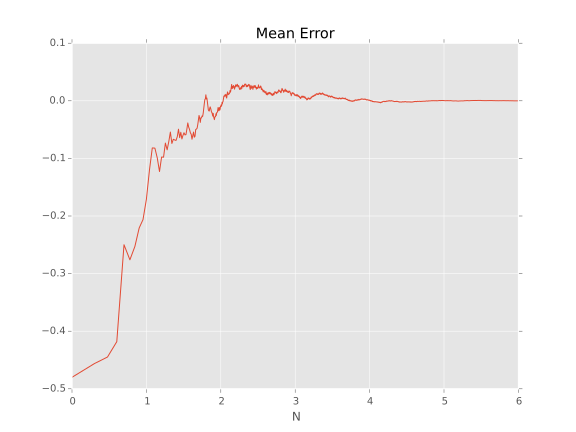
\includegraphics[width=\linewidth]{figure_1}
	\caption{2 dimensional uniform distribution.}
	\label{fig: 2du} 
\end{figure}

As expected, the distribution is flat. The illustration does exhibit slight distortion from the expected shape due the resolution provided by the small range of the plot's axes. The variance of the PDF confirms the ``flatness'' of the plot. $\sigma = 2.62 \times 10^{-21}$.

\subsection{2 Dimensional Normal Distribution} 
The $\Re2$ multivariate normal distribution was generated utilizing a built in function \verb|multivariate_normal()| which is fed the length ($N$), dimension (2), and covariance matrix ($cov_k$). The output of the function is identical to the shape of $x$ described in the previous section, and therefore is treated also identically to illustrate in $\Re3$.  \\

To aid visualization, contour lines were added in addition to the surface plots. Two sets of plots were generated for covariance matrices, one consisting of both the surface and contour plots, and another consisting of only the contour plots. The result with $N = 1 \times 10^6$, $B = 25$, $\mu = (6,6)$ and the covariance matrices 1 to 5 can be seen below in figures~\ref{fig: 2dn} and \ref{fig: 2dnc}.
\begin{figure}[H] 
	\centering 
	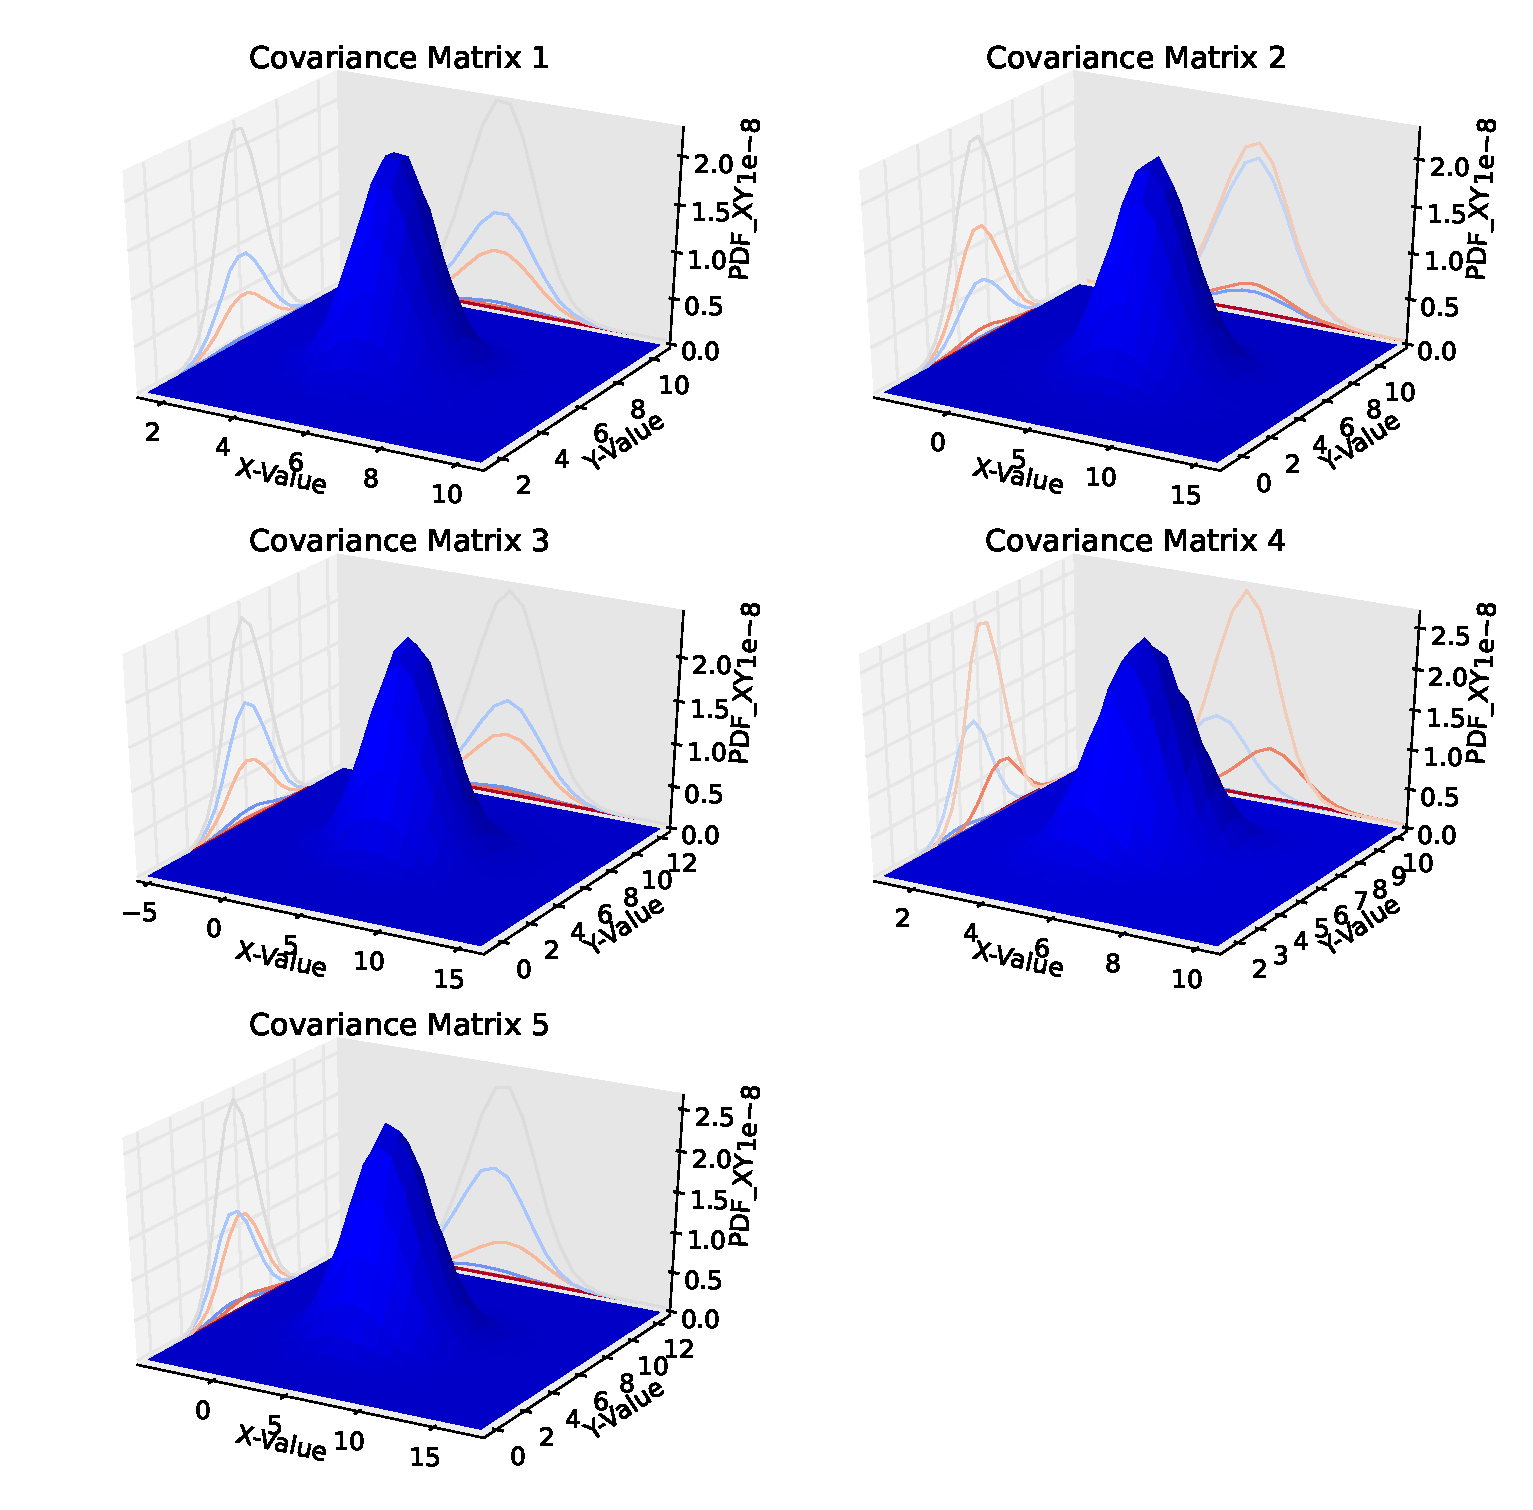
\includegraphics[width=\linewidth]{figure_2}
	\caption{2 dimensional normal distribution illustrated through surface and contour lines.}
	\label{fig: 2dn} 
\end{figure}

\begin{figure}[H] 
	\centering 
	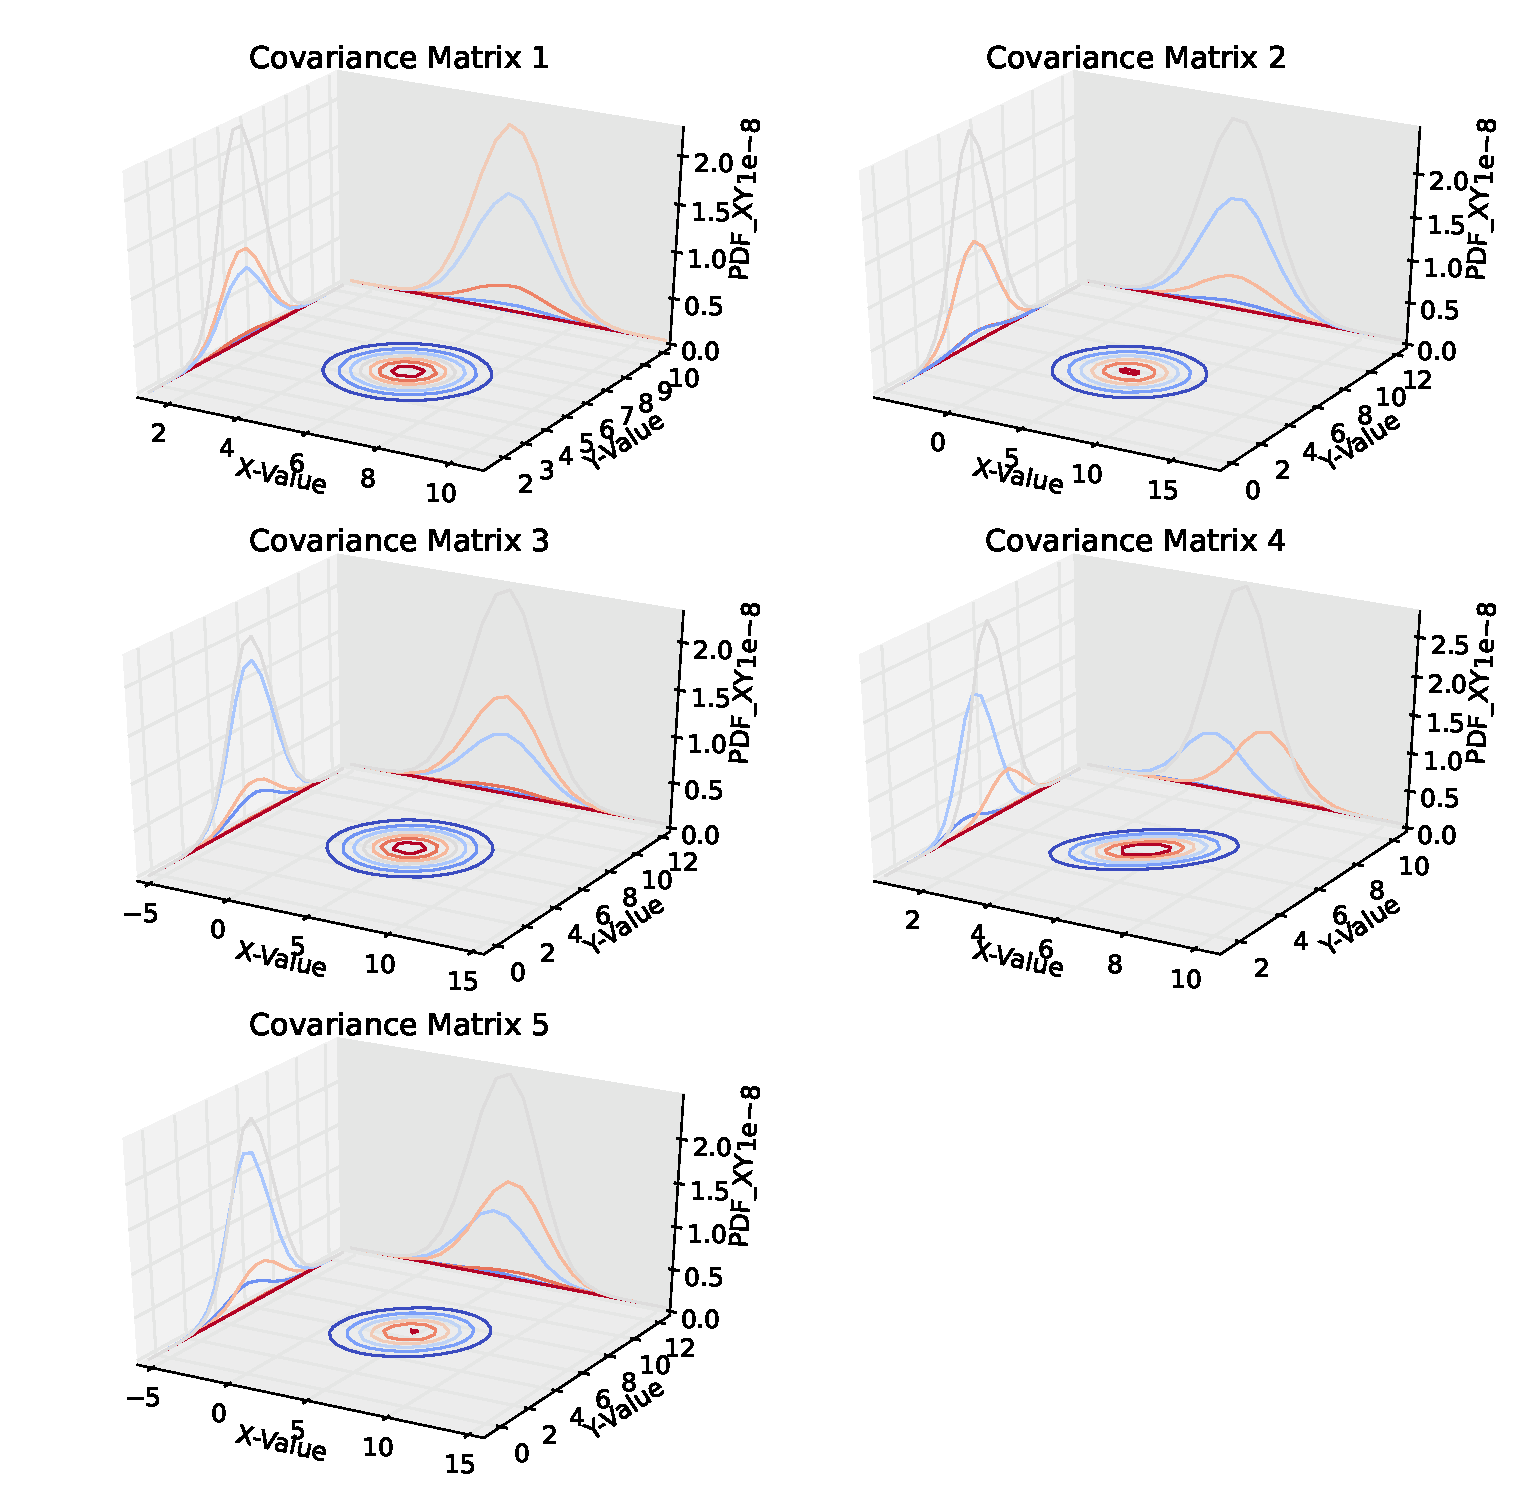
\includegraphics[width=\linewidth]{figure_3}
	\caption{2 dimensional normal distribution illustrated throughcontour lines.}
	\label{fig: 2dnc} 
\end{figure}

$cov_1$ and $cov_2$ are identical matrices, but their multivariate distributions are clearly different in there range of possible values. There shape is nearly identical as displayed by the contour lines with a circular base and symmetrical Gaussian projections on the $XZ$ and $YZ$ plane. For matrix $cor_3$ the distribution's projections on the $XY$ plane are still circular, but the projections on the $XZ$ are $YZ$ are no longer symmetrical to each other. There is a higher tendency and a wider range for $X$ compared to $Y$.   \\

For the matrices $cor_4$ and $corr_5$ the distribution's projections are not symmetrical in the $XZ$ and $YZ$ planes, and the projections in $XY$ plane are now elliptical. The matrices $cov_1$, $cov_2$, and $cov_3$ are all ``fundamentally identity matrices'' (Is there a word?) where the PDF of $X$ and $Y$ maintain independence in the distribution. This is not the case for $cov_4$ and $cov_5$. 
 
\section{Python Code} 
%Show and briefly explain your MATLAB code.
\lstinputlisting[caption=Script for task (1).]{../Python/ca_07_01.py}
\lstinputlisting[caption=Script for tast (2).]{../Python/ca_07_02.py}

\section{Conclusions} 
%Summarize what you found.
Visualizing data in $\Re3$ is entertaining. A two dimensional uniform uncorrelated PDF is flat. A two dimensional normal distribution which is uncorrelated has circular projection on the $XY$ plane. A two dimensional normal distribution which is correlated has an elliptical projection on the $XY$ plane.  

\end{document}